\documentclass[a4paper,12pt,twoside]{article}
\usepackage[T1]{fontenc}
\usepackage[utf8]{inputenc}
\usepackage{lmodern}
\usepackage[french]{babel}
\usepackage{url,csquotes}
\usepackage[hidelinks,hyperfootnotes=false]{hyperref}
\usepackage{enumitem}
\usepackage{amsmath}
\usepackage{graphicx}

\usepackage{caption}
\usepackage{subcaption}
\usepackage{float}


\title{Quantum Monte Carlo algorithm for spins systems}
\author{Etienne \bsc{Camphuis}}


\begin{document}
	\begin{titlepage}
		\begin{center}
			\textsc{\Large Digital Physics}\\[1.5cm]
			
			{ \huge \bfseries Quantum Monte Carlo algorithm for spins systems\\[0.4cm] }
		\vfill
		\begin{minipage}{0.4\textwidth}
			\large
			\centering
			Etienne \textsc{Camphuis}\\
			Barthélémy \textsc{Meynard Piganeau} \\
			X 2016\\
		\end{minipage}
		
		{\large December 2018, $7^{th}$}
		\end{center}
	\end{titlepage}
	
	\section{Local Algorithm}
	\subsection{description}

		
		 This section focuses on a way to move through the configurations.
		 The local Algorithm need to implement two distinct moves:
		 
		 \begin{itemize}
		 	\item{the splitline move} This move is supposed to inverse a complete line. To be implemented we firstly chose a spin, then check if the all the spins upward have the same value, and in that case invert all opf them.
		 	
		 	\item{the kink move} This move move represents the effect of the quantic spins. The part Jx and Jy create variation from the usual spin model. It is taken in account with this move, which flip the 4 spins around a black case, if the two left spins are the same and are the oposite of the two right spins.
		 \end{itemize}
		 	
		 	
		 	
		 	\subsection{domain of validity}
		 	\subsubsection{Winding number}
		 	It can not deal with periodic boundary conditions. Indeed, because the updates are either local or along a temporary line, the winding number is fixed. The winding number is an integer counting the number of period that the world-line takes to return to the same position. 
		 	\begin{figure}[!h]
		 		\centering
		 		
		 		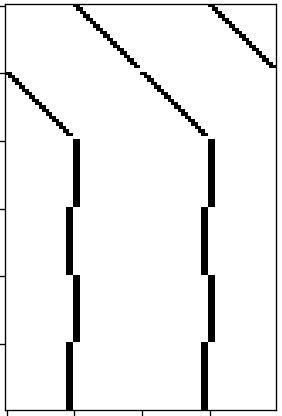
\includegraphics[]{Pattern_winding.png}
		 		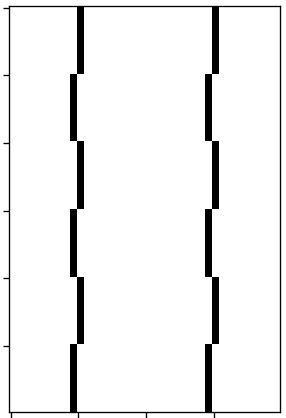
\includegraphics[]{Pattern_nowinding.png}
		 		\caption{Configurations with W = 2 (left) and W = 1 (right)}
		 		\label{winding}			
		 	\end{figure}
		 	
		 	
		 
		 
		 \subsubsection{straight line only can be flipped}
		 After a few attempts to split any world-line we only add wrong result. Indded we realized it caused an error in the detailed balance.
		 Indeed if we start from the following situation 1 and split the worldline 3 we get to the situation 2.
		 
		 \begin{figure}[!h]
		 	\centering
		 	\begin{subfigure}[b]{0.3\textwidth}
		 		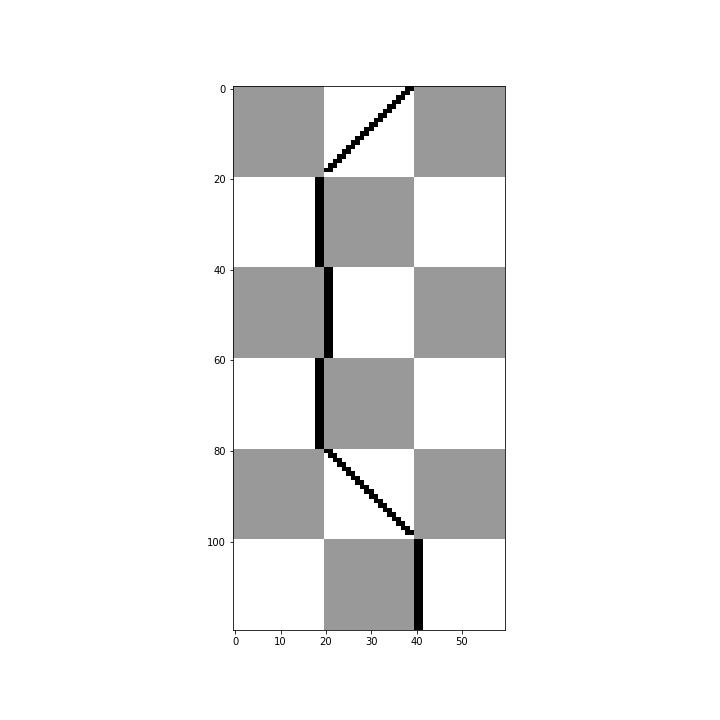
\includegraphics[scale=0.2]{situation1.png}
		 	\end{subfigure}
		 	\begin{subfigure}[b]{0.3\textwidth}
		 		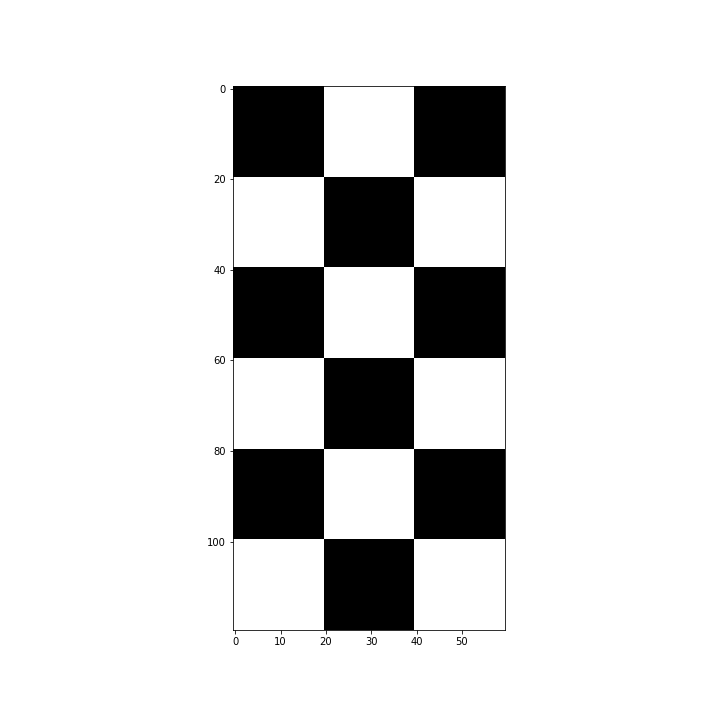
\includegraphics[scale=0.2]{situation2.png}
		 	\end{subfigure}
		 	\begin{subfigure}[b]{0.3\textwidth}
		 		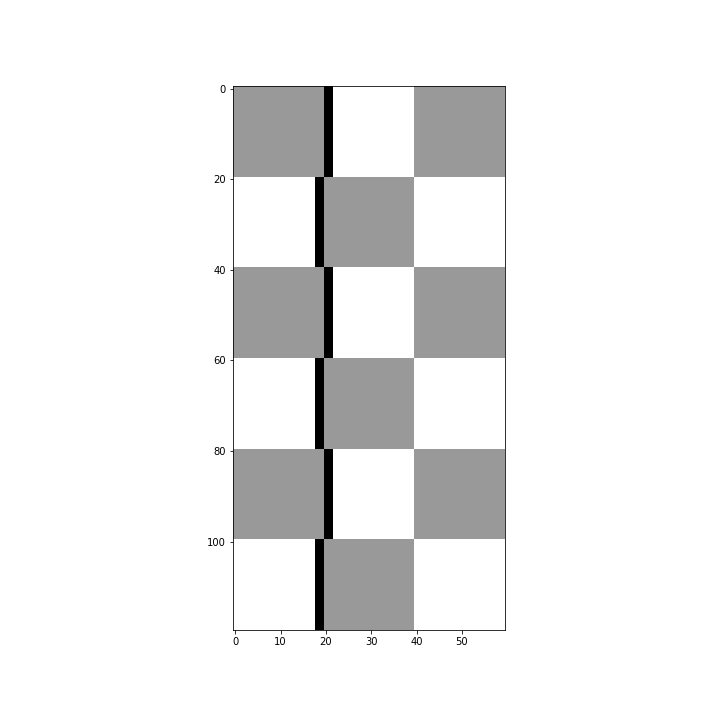
\includegraphics[scale=0.2]{situation3.png}
		 	\end{subfigure}
		 	\caption{situation 1 (left), situation 2 (middle), situation 3 (right)}
		 	\label{flawed detailed balance}			
		 \end{figure}
		 
		 From the situation 2 it is not possible to come back at the situation 1 with a simple splitline. Indeed such move only creates situation 3. To do so a splitline and a kink move is mandatory. The detailed balance is in this case unbalanced.
		 The solution is to accept to flip straight world-line only.
		 
		 To code a Monte Carlo algoriothm, we then had to condensed the two moves in one. We called it stoch\_move(threshold), this algo has a probability threshold to make a splitline move, and 1-threshold to make a kink move.
		 
		 
		 
		 
		 This algorithms 
		 \subsection{first results}
		 For the proper parameter the algorithm enable to compute the mean energy. In the following we'll focuse on the case $Jx = Jy = Jz =1, nspins = 4, beta = 1$.
		 Firstly we made a few run of the montecarlo algorithm, with a small length\_cycle (10) and a small number of measures(100 000), to have a first look.
		 
		 The found the following results:
		 \begin{itemize}
		 	\item theorical energy : -0.6330214400416617
		 	\item Energy for m=2: -0.6368988448758103 +/- 0.002502566964381992
		 	\item Energy for m=3: -0.6338973315707276 +/- 0.0027341143579975723
		 	\item Energy for m=4: -0.6229915669089899 +/- 0.002819998026568314
		 	\item Energy for m=5: -0.6445715838659634 +/- 0.0029559595617620286
		 	\item Energy for m=6: -0.6358614671234866 +/- 0.0029930079421800816
		 \end{itemize}
		 
		 At the first glance it seems that the algorithm give a good approxiamtion of the result. We firstly wanted to have an idea of the evolution of the mean energy with the number of measures.
		 \begin{figure}[!h]
		 	\centering
		 	
		 	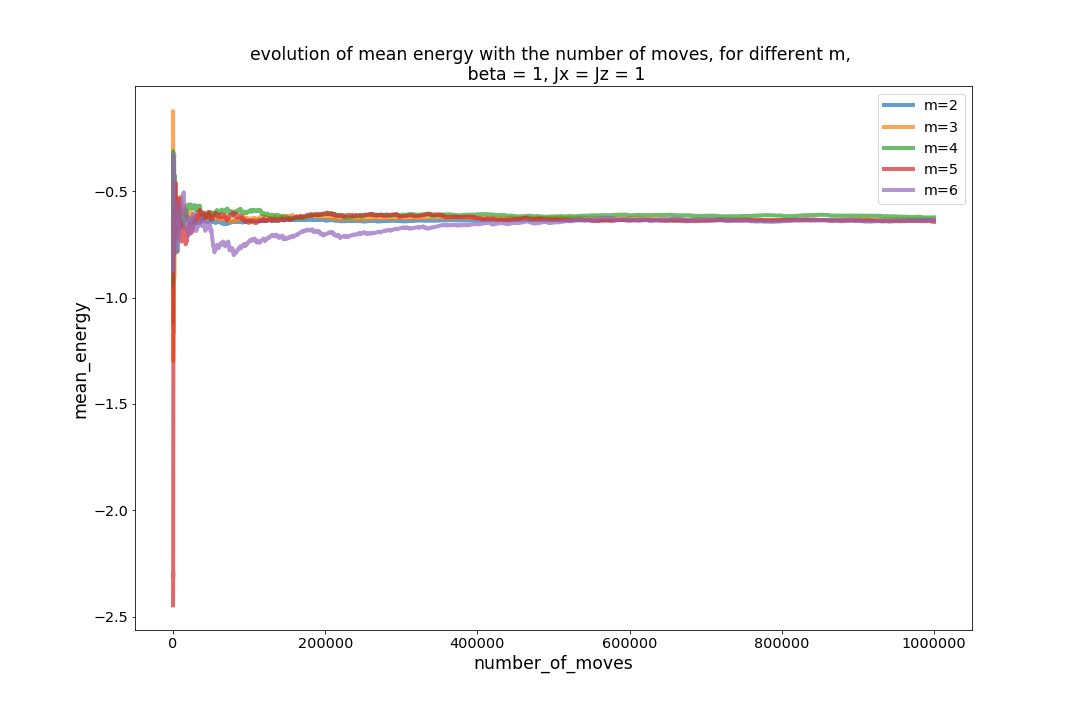
\includegraphics[scale=0.4]{meanenrgyevolution_x=z=1_m2-6.png}
		 	
		 	
		 	\label{energy mean evolution}			
		 \end{figure}
		 
		 We clearly feel that the 5 results converge to the same limit around -0.63. We also observe that the case m = 6 takes more moves to converge.
		 The beginning of the curves doesn't have much meaning. It has an high dependance regarding the initial configuration.
		 We can have a better look on the end of the graph:
		 
		 \begin{figure}[H]
		 	\centering
		 	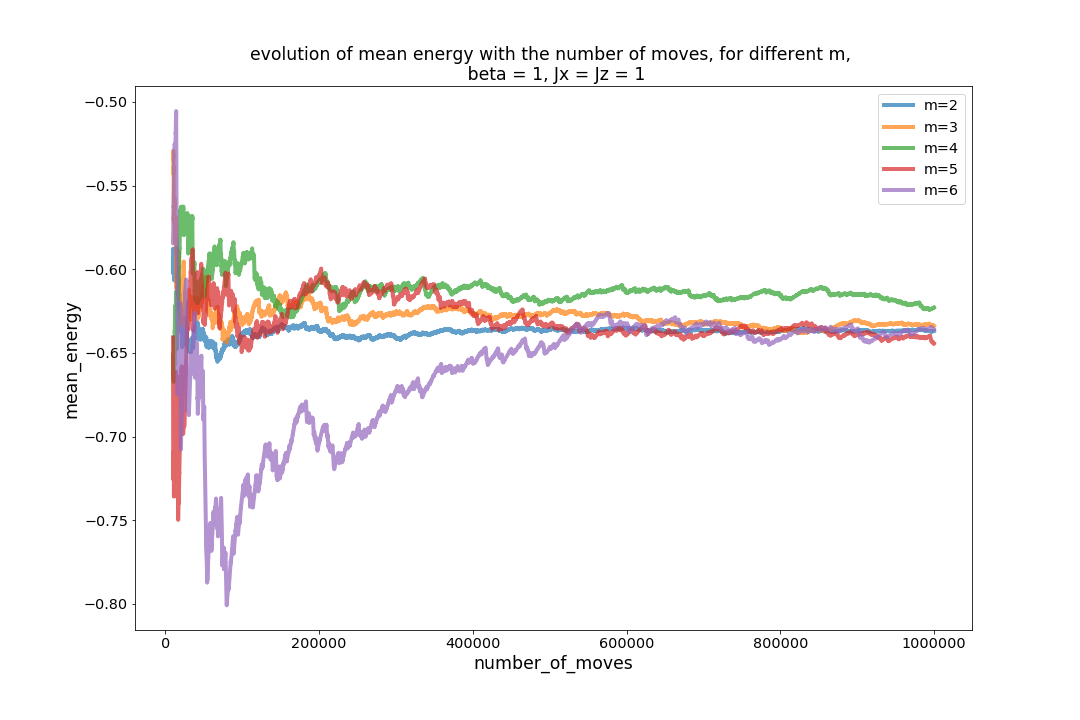
\includegraphics[scale=0.4]{mean_energy_evolution_centerd_x=z=1_m2-6.png}
		 	\label{energy mean evolution}			
		 \end{figure}
		 This graph enables us to see two things more clearly.  Firstly the number of moves necessary for the mean to converge rises with m. Secondly the choice of m seem to involve a bias in the mean.
		 While mtrotter rises, the number of configurations follows and the weight changed by the local\_update move decrease
		 
		 
		 \subsection{autocorrelation function}
		 To have a better idea of the length between two measures, we computed the autocorelation function. This function is defined for an observable O by the following formula
		 



	
	\subsection{limits}



	\section{Loop Algorithm}
	In this section, we will discuss the loop algorithm, introduced in the Assaad and Evertz article page 12. 
	
	\subsection{Failure of the local algorithm}
	The previous algorithm is not reliable for the three following reasons.
	


	\subsubsection{Acceptance rate} The rate of acceptance of the move is highly dependant on the parameters. For instance, should ...
	
	\subsubsection{Decorrelation} The decorrelation between the configuration is rather slow ...

	\subsection{The loop update}
	
	\subsubsection{Example}
	
	\paragraph{}The idea of Assaad and Evertz is to map the periodic boundary conditions model onto another one called "six-vertices model". Thanks to the result obtained on this model, we are now able to implement an update which allows fast decorrelation, high acceptance rate and changing winding number.
	Let us imagine each tile is replaced by its representation in the six-vertices model which is described in figure \ref{six_vertex}.
	\begin{figure}[!h]
		\centering
		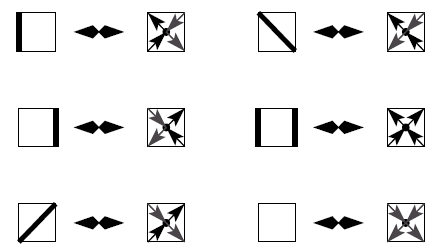
\includegraphics[]{six_vertex.png}
		\caption{Rule to change a tile in a vertex plaquette}
		\label{six_vertex}
	\end{figure}

	\paragraph{} The rule is the following : each spin up is transformed into an arrow going up; each spin down is transformed into an arrow going down. 
	Given this transformation one is now able to imagine loops on the pattern. One starts from a given spin and a given vertex plaquette, and go along the arrow in the same direction. If one does not choose two times the same arrow, he will come back to the first spin and thus create a loop. This mechanism is illustrated by the figure \ref{creating_loop}. The described loop "goes through" the right side to come back to the left side thanks to the periodic boundary conditions.
	\begin{figure}[!h]
		\centering
		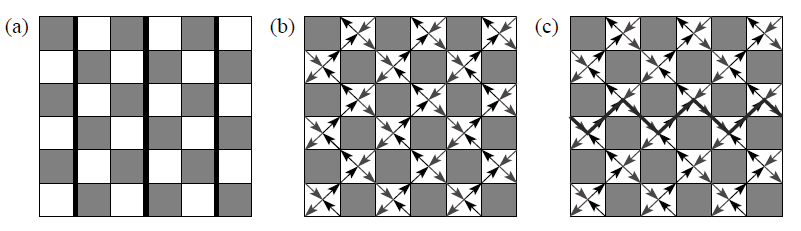
\includegraphics[]{creating_loop.png}
		\caption{Illustration of the creation of a loop}
		\label{creating_loop}
	\end{figure}

	\paragraph{}
	With the chosen loop, one can now flip the spins along the loop, which corresponds to changing the direction of all the arrows. This generates a new configuration. In the described one in figure \ref{creating_loop} and figure \ref{loop_update}, the winding number is changed from 1 to 3. One can observe that even this quite simple update (only one loop has been studied), the new configuration seems less dependant that any other that would have been generated thanks to the local algorithm. 
	\begin{figure}[!h]
		\centering
		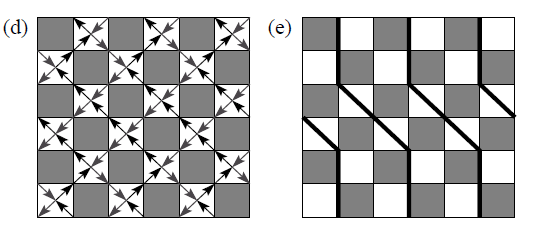
\includegraphics[]{loop_update.png}
		\caption{Update by flipping the spins along the loop}
		\label{loop_update}
	\end{figure}

	\subsubsection{Formalism}
	\emph{For the quantum Monte-Carlo algorithm, the detailed balance must be fulfilled. For a given tile in the configuration $S$, and for any other tile $S'$, the detailed balance is given by equation (\ref{detailed_balance})}
	\begin{equation}
		\centering
		W(S)P(S\rightarrow S') = W(S')P(S'\rightarrow S)
		\label{detailed_balance}
	\end{equation}
	
	\paragraph{}
	In order to make a move on the configuration, one has to change all the tiles in vertex plaquettes, then to choose loops and to choose whether to flip the spins along it or not. The process is clearer if one creates a virtual configuration called graph. For each tile, the associated vertex plaquette will be replaced by a graph-tile representing the choice of the arrows. The choices are either the loop goes vertically, either diagonally, either horizontally along the tile. Actually, there is another graph possible which switch all the spins on the tile, but it will not be considered here. Summing all the graph will create loops on the configuration. Figure \ref{graph_example} is an example of total graph
	\begin{figure}[!h]
		 \centering
		 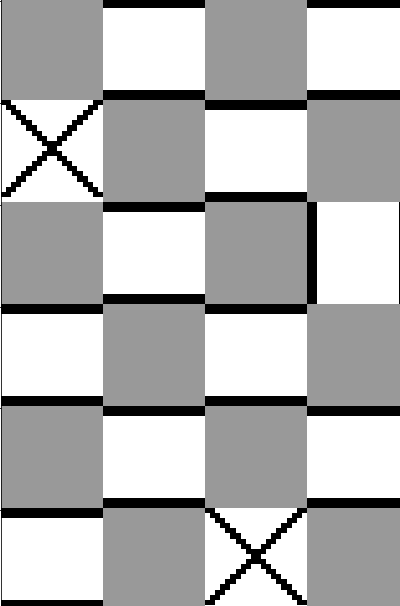
\includegraphics[width = 5cm]{random_graph.png}
		 \caption{Example of graph; one can verify that all loops are closed}
		 \label{graph_example}
	\end{figure}

	\paragraph{}
	First of all, one needs to know which graphs can be reached by a given tile. Let us give an example for the tile with all the spins down, the white tile. The associated vertex plaquette is the one with all the arrow heading down. If the loop arrives from the upper left side of the tile, it can either go to the bottom left or to the bottom right. Thus, only 2 graphs are allowed: either a vertical graph or a cross graph. The illustration is given in figure \ref{possible_graphs} for all tiles, one can verify the association following the previous logic applied to the white tile.
	\begin{figure}[!h]
		\centering
		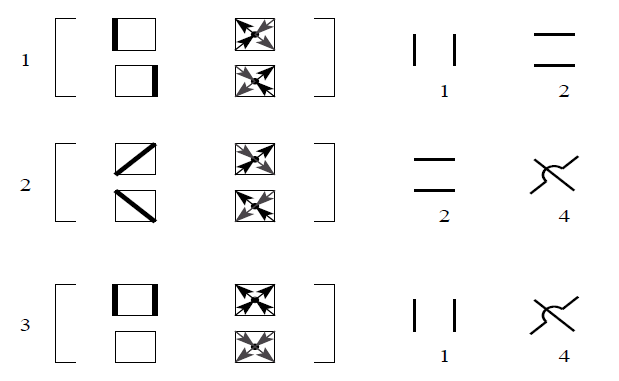
\includegraphics[]{possible_graphs.png}
		\caption{Possible graphs for tiles}
		\label{possible_graphs}
	\end{figure}

	\paragraph{}
	However, depending on the interactions and the temperature, the graphs will not be equally possible. One has to choose weights for each of them. Let us call $W(S)$ the weight of the tile $S$ and $W(S,G)$ the weight of the graph $G$ for a tile $S$. The equation (\ref{sg=s}) is required to have a total probability equal to one, and then be sure that every tile is replaced by a graph.
	\begin{equation}
		\centering
		\label{sg=s}
		\sum_{G}^{} W(S,G) = W(S)
	\end{equation}
	So we choose a graph from a given plaquette with probability
	\begin{equation}
		\centering
		P(S\rightarrow(S, G)) = \frac{W(S,G)}{W(S)}
		\label{psg}
	\end{equation}
	The detailed balance written with the graph transition
	\begin{equation}
		\begin{split}
			W(S)\sum_{G}P(S\rightarrow (S,G))P((S,G)\rightarrow(S',G))
			= \\ W(S') \sum_{G'} P(S'\rightarrow (S',G'))P((S',G')\rightarrow(S,G'))
		\end{split}
		\centering
	\end{equation}
	By using equation (\ref{psg}) is can be rewritten
	\begin{equation}
		\begin{split}
		\sum_{G}W(S,G)P((S,G)\rightarrow(S',G)) = \\ \sum_{G'}W(S',G')P((S',G')\rightarrow(S,G'))
		\end{split}
		\centering
	\end{equation}
	Then one can choose the different parameters to make the computation easier. For instance, the weights of the graph is set constant, not dependant on the spin configuration. This is easier to encode and clearer for the detailed balance:
	\begin{equation}
		\centering
		\forall G, \forall(S,S'), W(S,G) = W(S',G) = V(G) \label{indepG}
	\end{equation}
	 Moreover, with the use of the heat-bath algorithm for flipping, the probability to change the spin from $S$ to $S'$ given a choice of graph $G$ can be set to $P((S,G)\rightarrow(S',G)) = \frac{W(S',G)}{W(S',G) + W(S,G)}$. Thus the detailed balance is verified and the code is easy to encode. Indeed
	\begin{equation}
		\begin{split}
			P((S,G)\rightarrow(S',G)) & = \frac{W(S',G)}{W(S',G) + W(S,G)} \\ & = \frac{V(G)}{V(G) + V(G)} \\ & = \frac{1}{2}
		\end{split}
		\label{onehalf}
	\end{equation}
	The equation (\ref{onehalf}) means that each loop is flipped with probability $1/2$.\newline
	To set the weights of the graphs $V(G)$, equations (\ref{sg=s}) and (\ref{indepG}), with the use of the notations of figure \ref{possible_graphs} give
	\begin{equation}
		\left \{ \,
			\begin{split}
			W( S = 1 ) = V( G = 1 ) + V( G = 2 )
			\\
			W( S = 2 ) = V( G = 2 ) + V( G = 4 )
			\\
			W( S = 3 ) = V( G = 1 ) + V( G = 4 )
			\end{split}
		\right.
		\label{systemsg}
	\end{equation}
	This set of equation (\ref{systemsg}) has the solution:
	\begin{equation}
		\left \{ \,
		\begin{split}
			V( G = 1 ) = \frac{1}{2}[W( S = 1 ) + W( S = 3 ) - W ( S = 2 )]
			\\
			V( G = 2 ) = \frac{1}{2}[W( S = 1 ) + W( S = 2 ) - W ( S = 3 )]
			\\
			V( G = 4 ) = \frac{1}{2}[W( S = 2 ) + W( S = 3 ) - W ( S = 1 )]
		\end{split}
		\right.
	\label{solutionsg}
	\end{equation}
	Then, the weights $W(S)$ are 
	\begin{equation}
		\left \{ \,
			\begin{split}
			&W( S = 1 ) = \exp(\Delta \tau J_{z}/4)\cosh(\Delta\tau J_{x}/2)
			\\
			&W( S = 2 ) = \exp(\Delta \tau J_{z}/4)\sinh(\Delta\tau J_{x}/2)
			\\
			&W( S = 3 ) = \exp(- \Delta \tau J_{z}/4)
			\end{split}
		\right.
		\label{reminderws}
	\end{equation}
	The weights of each graph is now set. All the problem is characterized and the implementation is possible. However, the $Metropolis$ algorithm is valid only for positive weights for $W(S)$ and $V(G)$. This fixes conditions on $J_{z}$ and $J_{x}$.
	With the condition $V(G=2) > 0$:
	\begin{equation}
		\begin{split}
		&\exp(\Delta \tau J_{z}/2)\sinh(\Delta\tau J_{x}/2) + \exp(\Delta \tau J_{z}/2)\cosh(\Delta\tau J_{x}/2) - 1  > 0 \\
		&\exp(\Delta \tau J_{z}/2)\exp(\Delta\tau J_{x}/2)  > 1\\
		&J_{x} > - J_{z}
		\end{split}
	\end{equation}
	With the condition $V(G=4) > 0$:
	\begin{equation}
		\begin{split}
		&\exp(\Delta \tau J_{z}/2)\sinh(\Delta\tau J_{x}/2) + 1 - \exp(\Delta \tau J_{z}/2)\cosh(\Delta\tau J_{x}/2) > 0 \\
		&\exp(- \Delta \tau J_{z}/2)  > \exp(- \Delta\tau J_{x}/2)\\
		&- J_{z} > - J_{x}\\
		& J_{x} > J_{z}
		\end{split}
	\end{equation}
	The final condition is then
	\begin{equation}
		\centering
		J_{x} > |J_{z}| > 0
	\end{equation}
	If ever $|J_{z}|$ is higher than $J_{x}$, the algorithm can be implemented with another type of graph, called $G = 3$, that propagates the loop along all the arrows, which means all the spins on the tile are flipped. This is a graph accessible by all the vertex plaquettes, which allows a new system (\ref{systemsg}) and a supplementary degree of freedom to set the weights $V(G)$. This option will not be considered in our algorithm.
	
	\subsection{Encoding the loop algorithm}
	The whole methods will be encoded in an algorithm
	
	\subsubsection{Parameters}
	
	\paragraph{}
	First, we create a class containing the necessary parameters. 
	\begin{itemize}[label=$\star$]
		\item The interactions $J_{x}$ and $J_{z}$
		\item The number of spins $n\_spins$
		\item The division of the imaginary time $m\_trotter$ and $\Delta\tau$
		\item The representation of the spins $spins$
		\item The pattern configuration $pattern$
		\item The graph configuration $total\_graph$
		\item The list of energies depending on the concerned tile $energymatrix$
		\item The list of tile weights depending on the concerned tile $weightmatrix$
		\item The list of arrays imaging the tiles $cases$
		\item The list of arrays imaging the graphs $graphs$
		\item The graph weights depending on the graphs $w11, w12, w22, w24, w31, w34$ 
	\end{itemize}
	
	\subsubsection{Methods}
	Here are the methods used in the Quantum Monte Carlo algorithm. 
	\begin{itemize}[label=$\star$]
		\item $total\_energy()$ : Thanks to array combination and the use of masks, this methods extract the energy of each tile on the pattern then sum those energies.
		\item $weight()$ : Thanks to array combination and the use of masks, this methods extract the weight of each tile on the pattern then make the product of those weights to return the full weight of the combination.
		\item $spins\_to\_pattern()$ : With the use of array combination, this method computes the pattern from the spin configuration. At each coordinate $(i,j)$ is a number corresponding to the tile.
		\item $createimage()$ : Returns an array imaging the total world-line pattern.
		\item $tile\_in\_graph(pos)$ : Chooses a graph for the tile in position \\ $(pos[0], pos[1])$ with probability $\frac{V(G)}{W(S)}$.
		\item $set\_total\_graph()$ : Goes over the whole parameter $total\_graph$ and choose for each position a graph thanks to the previous method \\ $tile\_in\_graph(pos)$. An example of transformation is given is the figure \ref{tileandgraph}.
		\begin{figure}[!h]
			\centering
			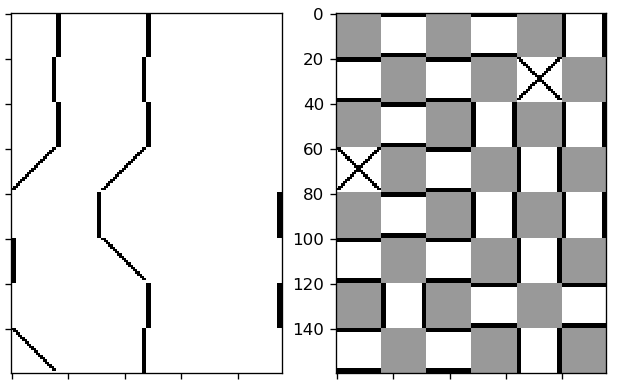
\includegraphics[]{tileandgraph.png}
			\caption{Example of transition from a given pattern to a graph}
			\label{tileandgraph}
		\end{figure}
		\item $find\_next(pos, graph)$ : This method is used to get the loops from the graph. The $pos$ and $graph$ parameters corresponds respectively to the position of a spin and the one of a graph. The method returns a new spin position and a new graph position after propagating the loop through the given $graph$ from the $spin$ position. For instance, if the graph is $G = 1$, $i.e.$ vertical, and the spin is on the upper left side on the graph, the method will return the spin just below the first spin and the graph down left the first graph. 
		\begin{figure}[!h]
			\centering
			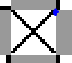
\includegraphics[]{firstgraph.png}
			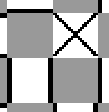
\includegraphics[]{twograph.png}
			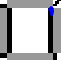
\includegraphics[]{secondgraph.png}
			\caption{Ensemble of two graphs; the left graph with the blue spin position will give the right graph with the blue spin position through $find\_next()$}
			
		\end{figure}
		\item $find\_loops()$ : This method will find all the loops and flip them with probability $\frac{1}{2}$. It goes over all the spin, and when any spin is not already in a loop, is uses the method $find\_next()$ to know the following spin in the associated loop, thus until is goes back to the same spin. At each step, is stores the spin to know which spins have already been treated. \\
		When it finds a not treated spin, it chooses with probability $\frac{1}{2}$ whether to flip all the spin along it or not. 
		\item $creategraph()$ : Returns an array imaging the total graph configuration.
		\item $pattern\_to\_string()$ : Transforms the $spins$ into a string to allow the script $check\_loop\_ergodicity.py$ to check if the algorithm is ergodic, i.e. that all configurations are reachable.
		\item $QMC\_step()$ : This method applies a step on the configuration. First, is computes the pattern from the spins. Then, it uses the computed pattern to set the $total\_graph$. Then, thanks to the $find\_loop()$ method it changes the spins to a new configuration.
		\item $Quantum\_Monte\_Carlo(n\_warmup, n\_cycles, length\_cycle)$ : This method uses the metropolis algorithm to compute the mean energy. First, the initial state with all spins down is "warmed up" by $n\_warmup$ cycles. Then, there are $n\_cycles$ cycles of $length\_cycle$ steps. For each cycle, the energy is measured once. The parameter $length\_cycle$ is used to get rid of the correlation between two successive configuration. This parameter can be optimize. 
	\end{itemize}
	
	\subsection{Results}
	
	\subsubsection{Case $J_{x} = J_{z}$}
	
	\paragraph{Parameters} For this case only, the graph $G = 4$ is not considered, because it's weight is null. 
	
	\paragraph{Validity of the algorithm} This case allowed us to check that our algorithm worked well with simple parameters.
	We used our code $ExactComputation$ to know the theoretical values for the following parameters: $J_x = J_z = - 1$,  $m\_trotter = 10$,  $N\_spins = 8$. The results for the Quantum Monte Carlo are computed thanks to the script $testloop.py$. \\
		\begin{tabular}[c]{| c || c | c |}
			\hline
			$\beta$ & Theoretical mean energies & Monte Carlo computed mean energies \\ \hline
			$0.1$ & $-0.146105$ & $-0.175369 \pm 0.045031$ \\ \hline
			$0.2$ & $-0.283938$ & $-0.318095 \pm 0.052067$ \\ \hline
			$0.3$ & $-0.412980$ & $-0.428188 \pm 0.047555$ \\ \hline
			$0.4$ & $-0.532973$ & $-0.550819 \pm 0.046009$ \\ \hline
			$0.5$ & $-0.643891$ & $-0.614586 \pm 0.039800$ \\ \hline
			$0.6$ & $-0.745901$ & $-0.775494 \pm 0.040258$ \\ \hline
			$0.7$ & $-0.839321$ & $-0.858818 \pm 0.039029$ \\ \hline
			$0.8$ & $-0.924584$ & $-0.912076 \pm 0.034779$ \\ \hline
			$0.9$ & $-1.002198$ & $-0.960219 \pm 0.035408$ \\ \hline
			$1.0$ & $-1.072715$ & $-1.081081 \pm 0.035624$ \\ \hline
		\end{tabular} 
	\newline
	This computation confirms that our code runs and produces the good results for parameters with $J_x = J_z$. This was tested for fairly few $n\_cycles$ in the Metropolis algorithm ($10000$), however it is sufficient.
	
	\paragraph{Ergodicity} In order to test our algorithm, we counted the number of different patterns that could be reached. If the algorithm is ergodic, is reaches all those patterns, that we are able to count. The script $check\_loop\_ergodicity.py$ allowed us to verify this property. 
	
	\paragraph{Autocorrelation}
	Let us show on figure \ref{meanenergylooplarger} the mean energy depending on the number of moves. We use the measures produced by the script \\ $compute\_x$=$z$=$1\_beta1.py$. Those are lists of $1e7$ measures for $J_x=J_z=1$ and $\beta=1$, but only the first 1000 moves are shown, it is on this time scale that the mean energy varies a lot. It can be seen that depending on the value of $m\_trotter$, the mean energy converges towards a different limit. This will be studied in the following paragraph. 
	\begin{figure}[!h]
		\centering
		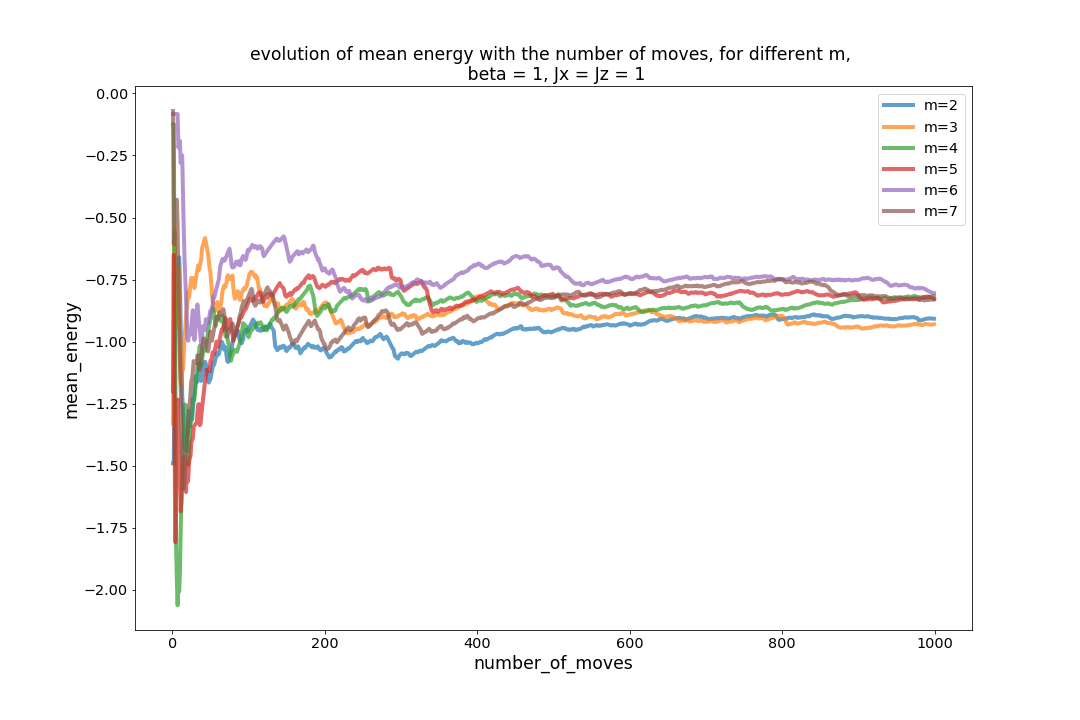
\includegraphics[width=12cm]{mean_energy_evolution_loop_x=z=1_m2-7.png}
		\caption{ }
		\label{meanenergylooplarger}
	\end{figure}
	The script $loop\_result.ipynb$ delivers the figure \ref{meanenergylooplarger} and \ref{autocorrloopxy}. The following figure directly computes the autocorrelation in the same way as in the local algorithm. One can observed that the autocorrelation is quite small, with an advised $length\_cycle$ at $10$.
	\begin{figure}[!h]
		\centering
		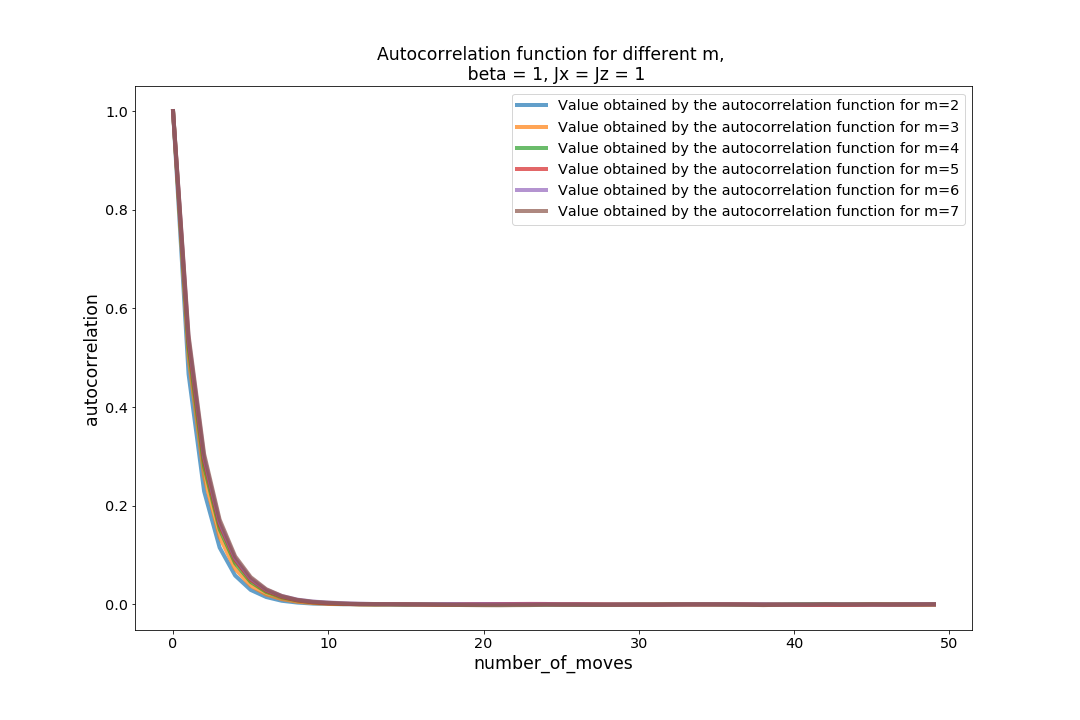
\includegraphics[width=12cm]{autocorr_loop_x=y.png}
		\caption{ }
		\label{autocorrloopxy}
	\end{figure}
	
	\paragraph{Result dependence on m}
	For a given number of spins and a given division of the imaginary time, there is a given number of configuration of the spins. Each has a weight. The Quantum Monte Carlo computation of the energy returns an energy than can be predicted for low values of $n\_spins$ and $m\_trotter$. Those predictable energies were given to us by M. Ferrero. \\ The parameters are :
	\begin{equation}
		\centering
		\begin{split}
			J_x = J_z = 1, & \beta = 1, n\_spins = 4 \\
			m & \in [2, 3, 4, 5, 6, 7] \\
			\Delta\tau & \in [\frac{1}{2}, \frac{1}{3}, \frac{1}{4}, \frac{1}{4}, \frac{1}{5}, \frac{1}{6}, \frac{1}{7}, ]
		\end{split}
	\end{equation}
	The following figure \ref{varymx=y}, given by the script $show\_ThvsComp.py$, shows the theoretical values for the energy on the orange dashed line. The energies are then computed by the loop algorithm with $1e7$ measures. The error-bars are shown.
	\begin{figure}[!h]
		\centering
		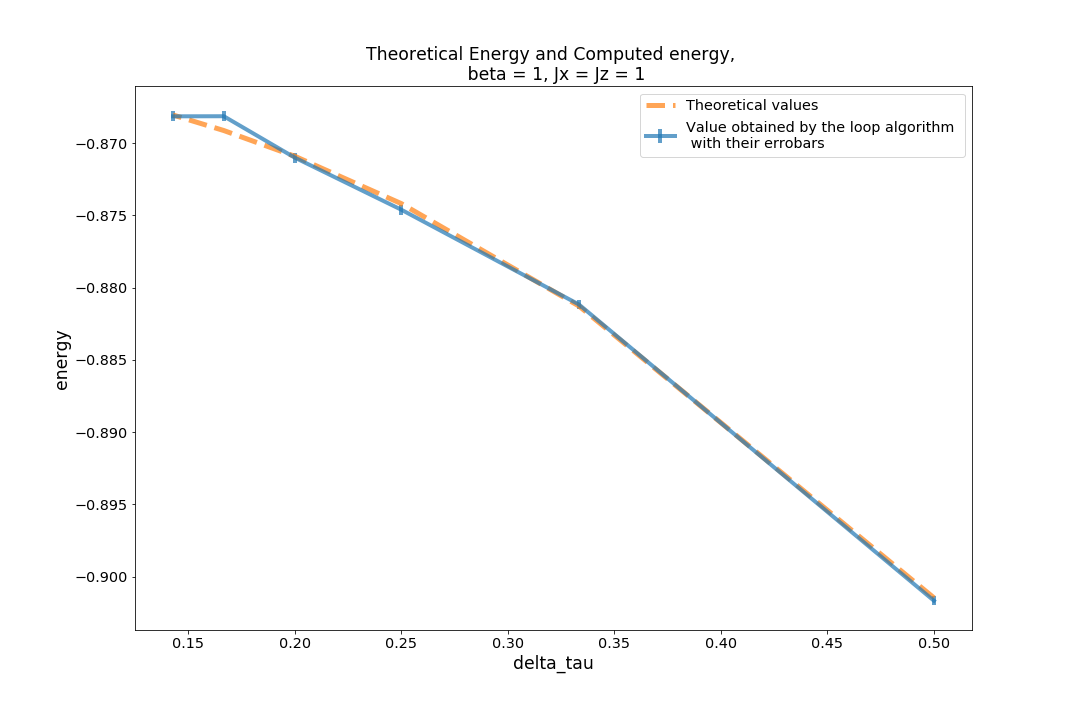
\includegraphics[width=12cm]{ThvsComp_x=z=1_m2-8.png}
		\caption{ }
		\label{varymx=y}
	\end{figure}
	
	\newpage
	\subsubsection{Case $J_{x} > |J_{z}$|}
	
	\paragraph{Parameters} For this case, all graphs are considered.
	\emph{During the encoding, because we faced difficulties, we tried to implement the code with another rule of repartition of the graphs' weights $V(G)$ such as the graph $G = 4$ was accessible only from the diagonal tiles $S = 2$ ($i.e.$ $W(S=3, G=4)=0$). This algorithm did not work, and the article written by Wessel that proposed such a repartition was wrong. Indeed, in this particular case, the detailed balance is not verified, as through the graph $G=4$, the tiles $S=2$ are transformed to $S=3$, and tiles $S=3$ can not reach tiles $S=2$.}
	
	\paragraph{Validity of the algorithm} We used our code $ExactComputation$ to know the theoretical values for the following parameters: $J_x = 1.0$, $J_z = 0.5$,  $m\_trotter = 10$,  $N\_spins = 8$. The results for the Quantum Monte Carlo are computed thanks to the script $testloop.py$. \\
	\begin{tabular}[c]{| c || c | c |}
		\hline            
		$\beta$ & Theoretical mean energies & Monte Carlo computed mean energies \\ \hline
		$0.1$ & $-0.114286$ & $-0.122148 \pm 0.014636$ \\ \hline
		$0.2$ & $-0.231759$ & $-0.255334 \pm 0.014792$ \\ \hline
		$0.3$ & $-0.351769$ & $-0.310946 \pm 0.013171$ \\ \hline
		$0.4$ & $-0.473585$ & $-0.487812 \pm 0.014690$ \\ \hline
		$0.5$ & $-0.596416$ & $-0.619067 \pm 0.014897$ \\ \hline
		$0.6$ & $-0.719437$ & $-0.747027 \pm 0.014502$ \\ \hline
		$0.7$ & $-0.841814$ & $-0.834654 \pm 0.013837$ \\ \hline
		$0.8$ & $-0.962735$ & $-0.936949 \pm 0.014312$ \\ \hline
		$0.9$ & $-1.081434$ & $-1.122287 \pm 0.014313$ \\ \hline
		$1.0$ & $-1.197217$ & $-1.149319 \pm 0.013671$ \\ \hline
	\end{tabular} 
	
	\paragraph{Other results}
	Due to time of computation, major results will be given during the oral.
	\newline
	
	\newpage
	\section{Conclusion}
	Thanks to the power of the loop algorithm, one can compute the mean energy with a very low $length\_cycle$ and a high acceptance rate. Quite rapidly, as shown in figure \ref{meanenergylooplarger}, the mean energy converges towards the limit. 
	
	


\end{document}